\chapter{Présentation du projet}

\section{Introduction}

La nature a donné à l’homme et aux animaux complexes des organes qui leur permettent d’interpréter les différentes informations de leur environnement. Ces organes peuvent capter des grandeurs physiques qui sont envoyées au cerveau pour pouvoir interpréter les changements dans le monde qui nous entoure ; ce sont les sens. L’un des phénomènes physiques capté par nos organes est “les ondes”, tantôt mécaniques avec l’ouïe, tantôt électromagnétiques avec la vue, qui constituent les deux principaux sens de l’homme. Or ces sens ne captent qu’une infime partie de tout le spectre existant des ondes. \\
Malheureusement ces sens peuvent être endommagés, ce qui devient une contrainte pour la personne affectée. Selon \acrfull{who}, environ 1,3 milliard de personnes vivrait avec une forme de déficience visuelle \cite{WHO-blindness-and-visual-impairment}, où, approximativement, 49.1 million d'eux sont aveugles \cite{number-of-blind}. \\
Les personnes aveugles, ont beaucoup de difficultés non seulement pour se déplacer physiquement, en particulier dans des environnements qu'ils ne connaissent pas, et encore devant des obstacles qu’ils ne voient pas.

% Problématique et besoins

\section{Problématique et besoins}

Heureusement, il existe différentes techniques, outils et des technologies disponibles pour permettre aux handicapés de réaliser leurs activités quotidiennes, Un des outils les plus utilisés est la canne blanche qui permet à l’utilisateur de détecter des obstacles qui se trouvent à un mètre de lui environ et, également, de déceler l’état du sol sur lequel ils marchent. Cependant, il existe encore des déficiences pour détecter des obstacles plus hauts ainsi que pour toucher les obstacles et les reconnaître. La technologie des capteurs nous permet d’identifier des grandeurs physiques et de les transformer en informations grâce à la connaissance des phénomènes physiques qui y interviennent. La compréhension des ondes a permis de développer des capteurs qui peuvent détecter des objets à distance grâce à l’analyse des échos reçus.

Mais il reste encore le problème de déplacement, Les personnes aveugles sont les plus susceptibles de se perdre, car elles ne peuvent pas localiser les lieux en raison de leur manque de vue c’est pourquoi on a pensé à élargir la portée de la canne blanche, l’utilisation de la technologie nous a poussé à  introduire le GPS (Global Positioning System) , au premier lieu cette idée va sembler compliquée mais on a pensé à utiliser un système de navigation nous l’avons tous chez nous c’est le smartphone , Tous les smartphones commercialisés ces dernières années sont dotés d'une puce GPS et c'est grâce à celle-ci que votre téléphone peut être géolocalisé, c'est-à-dire que vous pouvez connaître sa position géographique, alors on va essayer de créer une liaison entre eux et la canne blanche pour qu’il nous aide à résoudre le problème de navigation chez les aveugles \\et pour rendre notre système plus parfait on va essayer de traiter d’autres problèmes qui rencontre les aveugles comme :
\begin{itemize}
    \item Perdre leurs cannes qui va être un problème sérieux car elle est la seule méthode de leurs navigations et cela le rend vulnérables aux accidents Ce qui les rend vulnérables aux accidents, et pire encore, les rendra devant le problème que nous avons mentionné plus tôt, qui est de se perdre dans un endroit qu'ils ne connaissent pas, et encore une fois on va utiliser le smartphone pour trouver la canne et vice versa. 
    \item la décharge d’un des composants (canne blanche, smartphone). 
    \item l’utilisation de smartphone, on ne doit pas oublier la faite que les aveugles vont trouver des difficultés a utiliser leurs smartphones notre rôle va être crée une méthode de communication entre les aveugles et leurs smartphones basée sur l’ouïe et le toucher.
\end{itemize}

\section{Les taches intelligents à réaliser}

Comme indiqué précédemment, les aveugles ont du mal à faire leurs tâches quotidiennes simples, sans parler de pouvoir d'aller dehors. Ce qui nous a fait réfléchir à la façon dont nous pouvons faciliter leur navigation. Alors que les objectifs de notre projet sont les suivants:
\begin{itemize}
    \item La détection des obstacles et leur proximité.
    \item Faciliter l’utilisation du téléphone pour la navigation et la rendre plus rapide et plus facile.
    \item Être en mesure de trouver leur canne égarée à l’aide de leur téléphone, et vice versa.
    \item Appeler à l’aide au cas où il serait perdu, et généralement faciliter l’information des autres de leur emplacement actuel.
    \item Trouver les différents lieux proches de lui, classés par catégories, et l’y conduire.
    \item Contrôler toutes ces tâches avec son téléphone et/ou sa canne.
    \item Avoir la possibilité de charger son téléphone avec la canne
\end{itemize}

\subsection{La détection d’obstacles}

Pour réaliser cette tache, on utilisera un capteur de proximité qui permet la détection d'obstacles et leur proximité.
À cause de son prix, sa portabilité, ainsi que sa précision et sa simplicité d'utilisation, on a choisi le modèle HC-SR04 à utiliser.

% Pour informer l'utilisateur qu'il y a un obstacle devant lui, on utilisera deux vibreurs, cités à chaque côté de la canne. L'intensité de vibration augmente avec la proximité d'obstacle.

\subsubsection{Le HC-SR04}

\paragraph{Description}
Le capteur de distance ultrasonique HC-SR04 est un capteur utilisé pour détecter la distance d’un objet à l’aide d’un sonar. Il est idéal pour tous les projets de robotique que vous avez qui vous obligent à éviter les objets, en détectant à quel point ils sont proches, vous pouvez vous éloigner d’eux \cite{piborg-hc-sr04}!

\paragraph{Avantages}
Le capteur est petit, facile à utiliser dans n’importe quel projet de robotique et offre une excellente détection sans contact entre 2 cm à 400 cm avec une précision de 3mm. Puisqu’il fonctionne sur 5 volts, il peut être raccordé directement à un Arduino ou tout autre microcontrôleur logique 5V.

\paragraph{Principe de fonctionnement}
\label{hc-sr04:fonctionnement}
Tout commence lorsqu’une impulsion d’au moins 10 µs (10 microsecondes) de durée est appliquée à la broche de déclenchement (Trigger). En réponse à cela, le capteur transmet une rafale sonore de huit impulsions à 40 KHz. Ce motif à 8 impulsions rend la « signature ultrasonique » de l’appareil unique, ce qui permet au récepteur de différencier le motif transmis du bruit ultrasonique ambiant.

Les huit impulsions ultrasoniques se déplacent dans l’air loin du transmetteur. Pendant ce temps, la broche Echo va HAUT pour commencer à former le début du signal d’écho-retour.

Dans le cas, si ces impulsions ne sont pas réfléchies en arrière, le signal Echo expire après 38 ms (38 millisecondes) et revient bas. Ainsi, une impulsion de 38 ms n’indique aucune obstruction dans la plage du capteur \cite{hcsr04}.

On peut calculer la distance entre le capteur et l'objet en utilisant la simple relation en fonction de la vitesse du sons et la durée de déclenchement: \[d=\frac{v \cdot t}{2} \ \text{où} \ v \approx 340 m/s\]

En devise par 2 car le temps \(t\) est le temps d'aller-retour.


\begin{figure}[hbt!]
    \centering
    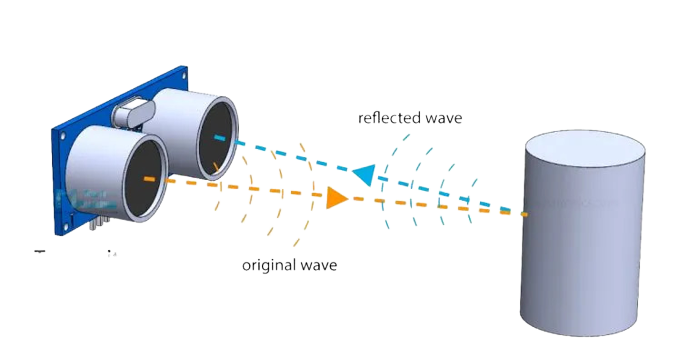
\includegraphics[width=14cm]{assets/HC-SR04/principe 3d.png}
    \caption{Principe du fonctionnement du HC-SR04}
\end{figure}

\begin{figure}[hbt!]
    \centering
    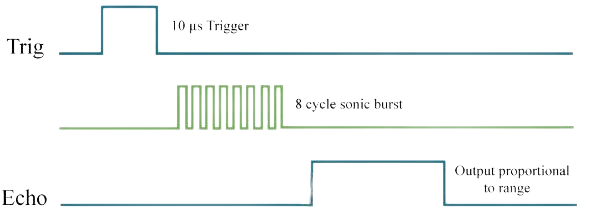
\includegraphics[width=14cm]{assets/HC-SR04/principe.png}
    \caption{Les signales de commande et de réponse du HC-SR04}
\end{figure}

\begin{figure}[!htbp]
    \centering
    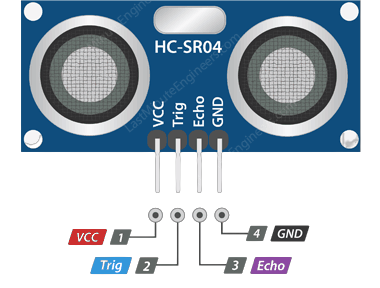
\includegraphics[width=10cm]{assets/HC-SR04/pinout.png}
    \caption{Brochage du module SR-HC04}
\end{figure}

\FloatBarrier

\subsubsection{Vibreur}

Pour informer l'utilisateur qu'il y a un obstacle devant lui, on utilisera deux vibreurs, cités à chaque côté de la canne. L'intensité de vibration augmente avec la proximité d'obstacle.

\begin{figure}[!htbp]
    \centering
    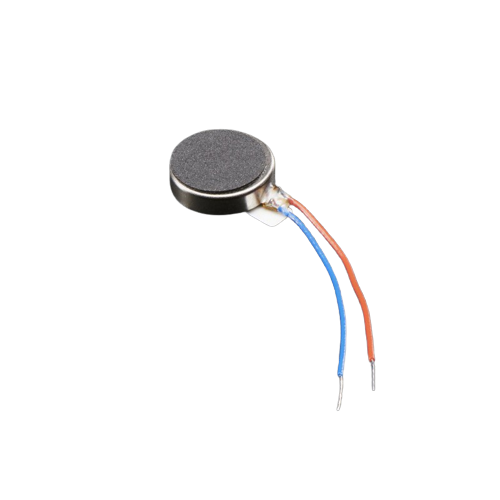
\includegraphics[width=8cm]{assets/vibrator.png}
    \caption{Moteur Vibreur}
\end{figure}

\FloatBarrier

Ce type de vibreurs nécessite 60mA et 5V pour bien fonctionner, main l'Arduino nano a une limitation de 40mA par broche, d'où on a besoin d'un motor driver.

\subsubsection{Motor Driver L293D}
Le circuit intégré L293D permet de piloter 2 moteurs à courant courant continu dans les deux sens de rotation et pour faire de la variation de vitesse.

\begin{figure}[!htbp]
    \centering
    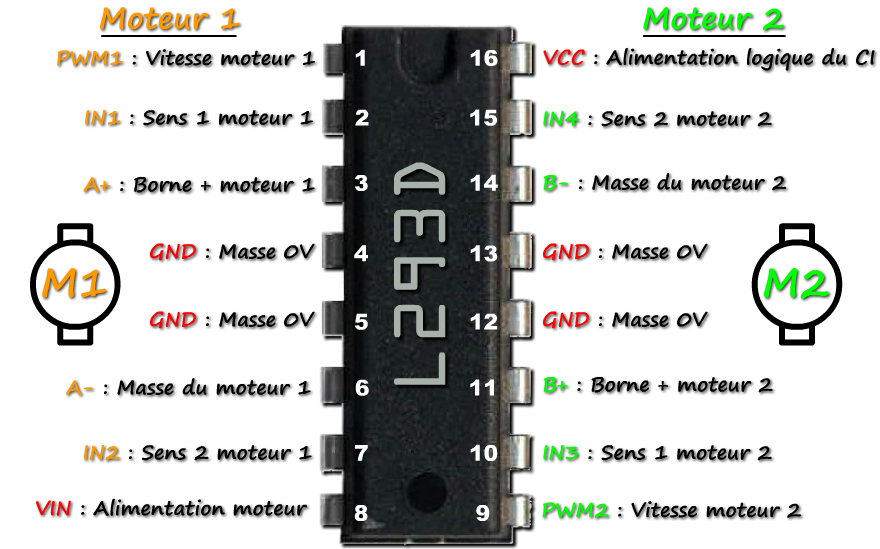
\includegraphics[width=13cm]{assets/L293D/pinout.png}
    \caption{Brochage du driver moteur L293D \cite{l293d-electrotoile}}
\end{figure}

\FloatBarrier

Pour notre projet, on n'a pas besoin de tourner le moteur à deux sens, donc on peut utiliser jusqu'à 4 moteurs.

\subsection{La navigation}

Pour aider l’utilisateur lors de la navigation, nous allons créer une application mobile multi-plateforme.
L’application aidera l’utilisateur à trouver des endroits qu’il connaît déjà, ou à découvrir des endroits à proximité de différentes catégories : Restaurants, mosquées, magasins et services, même les médecins et les pharmacies. Et si jamais il a aimé un endroit, il peut l'ajouter comme une place favourite pour qu'il puisse le retrouver simplement la prochaine fois.\\
L’application sera également responsable de guider l’utilisateur à sa destination, en utilisant Google Places API, et l’application Google Map.\\
Il sera également utilisable mains libres, juste par les boutons sur la canne. \\
La communication entre la canne et l'application mobile sera conduite par Bluetooth, en utilisant le module HC-05.

\subsubsection{Le HC-05}

\paragraph{Description}
Le module HC-05 est un module Bluetooth SPP (Serial Port Protocol), ce qui signifie qu’il communique avec l’Arduino via la communication série

\begin{figure}[!htbp]
    \centering
    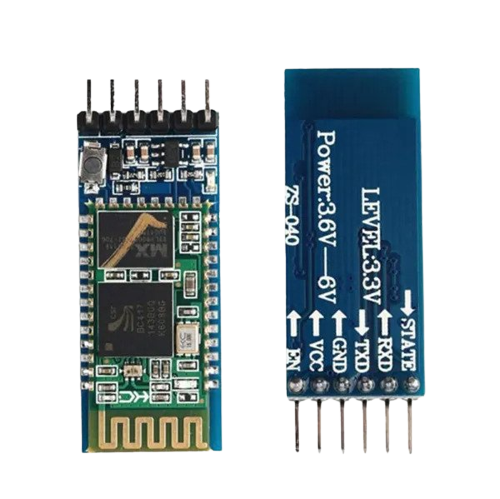
\includegraphics[width=8cm]{assets/HC-05/pinout.png}
    \caption{Module Bluetooth HC-05}
\end{figure}

\FloatBarrier

\paragraph{Brochage}\mbox{}\\
Le HC-05 consiste 6 broches:
\begin{itemize}
    \item VCC et GND: Pour l'alimentation +5V
    \item TXD et RXD: Pour la communication série
    \item State: Signifie si le module et connecter en Bluetooth ou pas. HIGH si oui, LOW si non.
    \item Enable: Broche de configuration, on la met a l'état HIGH pour avoir la possibilité de configurer le module (Nom, Mot de passe, Type ...) avec la communication série.
\end{itemize}

\subsection{Localisation de la place en cas de perte}

À l'aide de notre application, l'utilisateur aura la possibilité d'informer ses roches de sa position actuelle en utilisant le service GPS intégré à son smart-phone.\\
Sa localisation actuelle sera envoyée par un SMS aux contacts qu'il a déjà marqués comme contacts d'urgence, aussi que le message envoyer peut-être modifier simplement à l'aide de l'interface mobile.

\begin{figure}[!htbp]
    \centering
    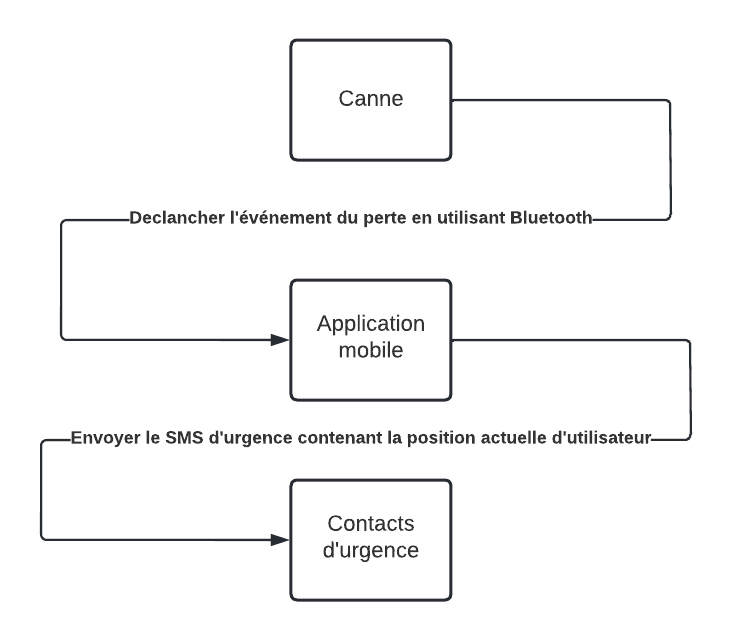
\includegraphics[width=.7\linewidth]{assets/principe d'envoie du SMS de perte.png}
    \caption{Cycle simplifié d'envoi du SMS au cas de perte}
\end{figure}

\FloatBarrier

\subsection{Trouver la canne en utilisant le téléphone et vice-versa}
Les personnes visuellement impayées ont du mal à trouver leurs objets, en particulier leurs téléphones. \\
Nous allons essayer d’éliminer ce problème en ajoutant la possibilité de commencer sonnerie de téléphone à partir de sa canne. Et ils peuvent également trouver leurs cannes en utilisant leurs téléphones en commençant une sonnerie sur la canne.

La sonnerie de la canne va être joue par le bipeur (Buzzer)

\subsubsection{Bipeur (Buzzer)}
\label{buzzer}
Un buzzer (anglicisme) ou bipeur est un élément électromécanique ou piézoélectrique qui produit un son caractéristique quand on lui applique une tension : le bip. Certains nécessitent une tension continue, d'autres nécessitent une tension alternative \cite{frwiki:178425382e}.

\begin{figure}[!htbp]
    \centering
    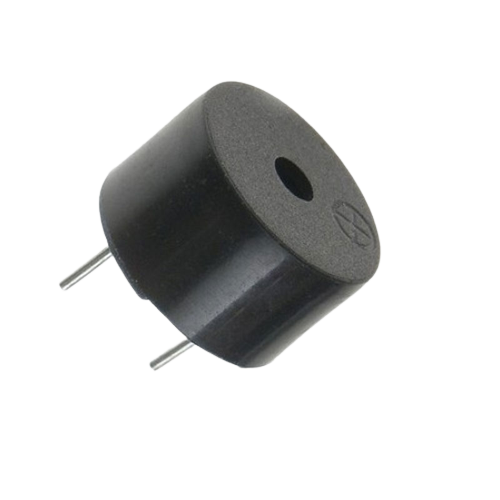
\includegraphics[width=8cm]{assets/buzzer.png}
    \caption{Buzzer}
\end{figure}

\FloatBarrier

\section{Arduino}

\subsection{C'est Quoi un Arduino ?}
Arduino est une plateforme électronique open-source basée sur du matériel et des logiciels faciles à utiliser. Cartes Arduino sont capables de lire les entrées - lumière sur un capteur, un doigt sur un bouton, ou un message Twitter - et de le transformer en une sortie - activer un moteur, allumer une LED, publier quelque chose en ligne. Vous pouvez dire à votre carte quoi faire en envoyant un ensemble d’instructions au micro-contrôleur de la carte \cite{arduino-introduction}.

\subsection{Les différents types d'un Arduino ?}
Les Arduinos sont caractérisés par plusieurs caractéristiques:

\begin{itemize}
    \item Processeur
    \item Vitesse d'horloge
    \item Tension d'entrée
    \item Tension de sortie
    \item Mémoire de stockage (Flash Memory)
    \item Mémoire vive (\acrshort{RAM})
    \item Nombre des pins entrée/sortie logique
    \item Nombre des pins entrée/sortie analogique
    \item Nombre des convertisseurs numérique/analogique (\acrshort{DAC})
    \item Nombre des pins supportant la modulation de largeur d'impulsion (\acrshort{PWM})
    \item Les différents protocoles de communication supportés (UART / SPI / I\(^2\)C)
    \item Type du connecteur
    \item Ses dimensions
\end{itemize}

Pour notre projet, on n'est pas très intéressé à toutes ses différentes caractéristiques, d'où on a créé un tableau qui compare les diffèrent types en se basant sur les caractéristiques qu'on a besoin.


\begin{table}[hbt!]
    \centering
    \begin{tabular}{|C{3cm}|C{2cm}|C{2.2cm}|C{2.2cm}|C{1.2cm}|C{1.5cm}|C{1.2cm}|}%|c|c|c|c|c|c|c|
        \hline
        &&&&&&\\ % Adding empty space on top of 0th column
        & Modèle & Vitesse d'horloge & Mémoire de programme & RAM & Nombre des pins & PWM \\[18pt]
        \hline
        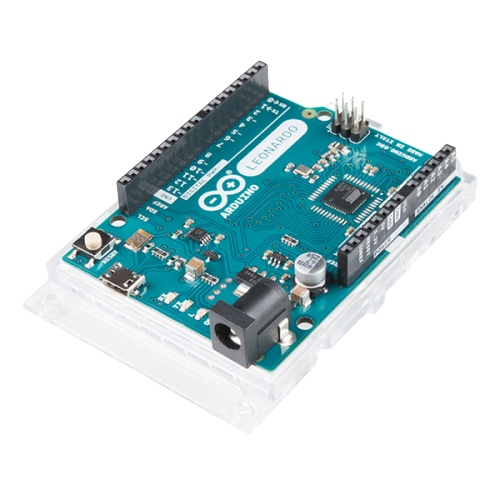
\includegraphics[width=3cm]{assets/arduino/leonardo.png} & UNO & 16MHz & 32KB & 2KB & 20 & 6 \\
        \hline
        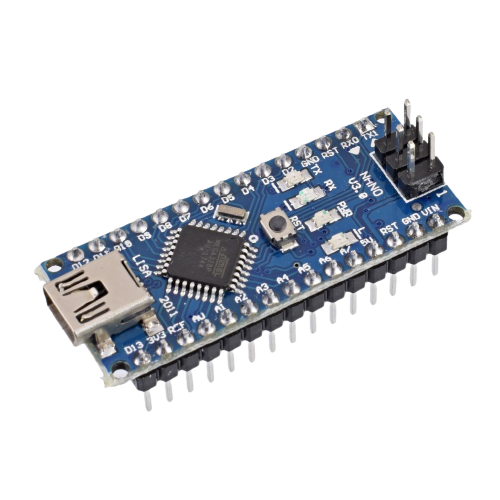
\includegraphics[width=3cm]{assets/arduino/nano.png} & Nano & 16MHz & 32KB & 2KB & 20 & 6 \\
        \hline
        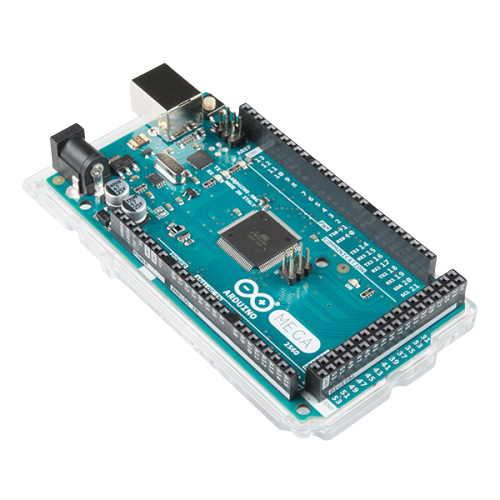
\includegraphics[width=3cm]{assets/arduino/mega.png} & Mega & 16MHz & 256KB & 8KB & 54 & 15 \\
        \hline
        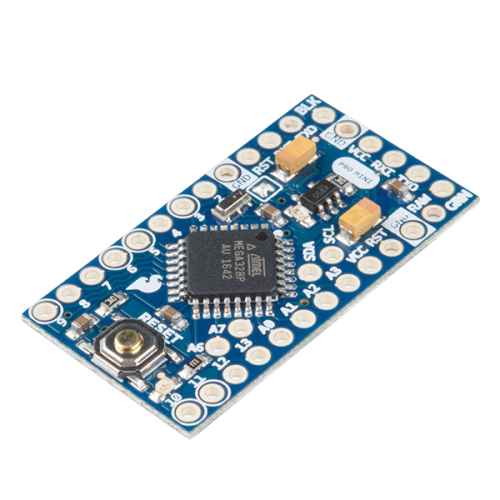
\includegraphics[width=3cm]{assets/arduino/pro mini.png} & Pro Mini & 8MHz & 32KB & 2KB & 22 & 8 \\
        \hline
        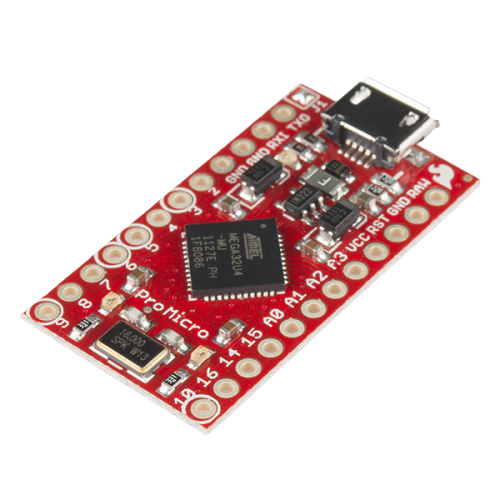
\includegraphics[width=3cm]{assets/arduino/pro micro.png} & Pro Micro & 16MHz & 32KB & 2.5KB & 18 & 5 \\
        \hline
        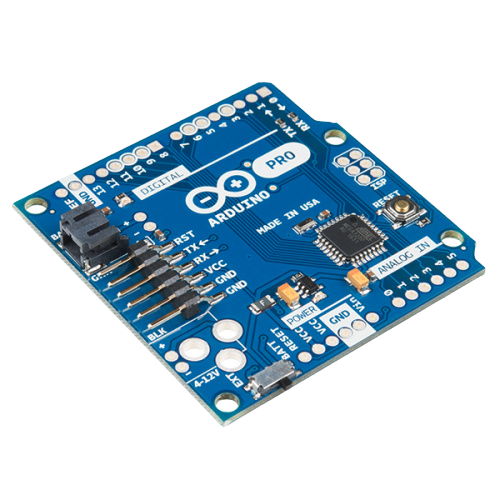
\includegraphics[width=3cm]{assets/arduino/pro.png} & Leonardo & 16MHz & 32KB & 2.5KB & 20 & 12 \\
        \hline
    \end{tabular}
    \caption{Les différents types d'Arduino \cite{arduino-types}}
\end{table}

\FloatBarrier

\subsection{Que-ce-qu'on a choisi?}

Notre projet a besoin de 14 entrées/sorties logiques, et une analogique. Où on avait le choix entre plusieurs modèles comme l'Arduino UNO, Nano, Pro Mini, et toute autre diffèrent type. Donc on avait pris autres caractéristiques en considération, surtout le prix et les dimensions, c'était indispensable d'avoir une qui peut être contenue dans un petit boîtier avec un bon prix. D'où on a choisi l'\textbf{Arduino Nano}, qu'il y avait des dimensions de 45 x 18 x 18 mm et un poids de 7g, à seulement 60DH.


\begin{figure}[hbt!]
    \centering
    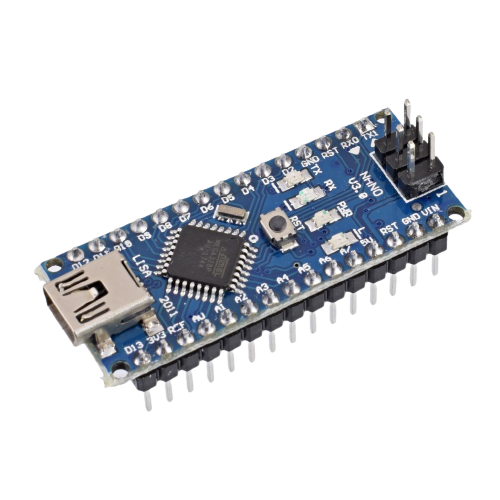
\includegraphics[width=5cm]{assets/arduino/nano.png}
    \caption{Arduino Nano}
\end{figure}

\section{Conclusion}

Maintenant et après qu’on a traité se système de différente partie et étudier un peu près tous les problèmes qu’il peut rencontrer, on peuvent réaliser ce projet commençant par les taches intelligents (La détection d’obstacles, La navigation, Localisation de la place en cas de perte, Trouver la canne en utilisant le téléphone et vice-versa), la réalisation du modèle de la canne, l’assemblage.